\chapter{Quantum digital signatures}
Goal of chapter: introduce our QDS protocol and prove its security in different contexts using several methods.

\section{Cryptography introduction}
%introduction and literature review
Goal of chapter: historical overview of development of quantum cryptography. Lead up to a thorough literature review for QDS, QSS and QKD.

Cryptography is a field probably as old as civilization itself. For as long as communication has existed, so too has the desire to keep information hidden. Both the Greeks and the Romans are known to have used ciphers to encrypt messages \MT{cite}. A cipher, after applied to a message, alows the encrypted message to be freely transmitted and intercepted without an adverse party knowing its meaning. The intended recipients, however, can undo the effects of the cipher and read the original message. \MT{It'd be cool to have an example of e.g. a ceasar cipher}.

Cryptanalysis--the art and science of breaking cryptographic systems--has existed for as long as cryptography. The history of cryptographic development can be viewed as a race between cryptographers and cryptanalysts. The cryptographers, Alice and Bob, continually invent new schemes to perform their secure communication task. The cryptanalyst, Eve, continually tries to break these schemes in order to interfere in Alice and Bob's communication.

\MT{The following segue seems quite abrupt}
There are two main important strands of cryptography: private-key and public-key crytography, Fig.~\ref{fig:pubpriv}. In private-key cryptography (also known as \emph{symmetric} cryptography), Alice and Bob share some secret information which they will use to perform some task, and without which an eavesdropper cannot break the system. An important example of private-key cryptography is encryption with a cipher $\mathcal{K}$ which is used to encrypt and decrypt messages. Any party with $\mathcal{K}$ can freely encypt or decrypt any piece of information, while any party lacking knowledge of $\mathcal{K}$ cannot. A relevant example of this type of cryptosystem is the one-time pad (OTP) which is discussed above.

\MT{Perhaps some discussion about how $\mathcal{K}$ can be distributed and attacked}

\MT{I should have a discussion at some point about how public- and private- key cryptography relate to each other and how they are both used in modern infrastructure}

The second strand is public-key cryptography (also known as \emph{asymmetric} cryptography). Here, there are several pieces of information required to run a protocol. Alice is assumed to hold a key $\mathcal{E}$ (her ``private key'') while Bob holds a key $\mathcal{D}$ (Alice's ``public-key'') which is assumed to be publicly known. As an example, Alice may encrypt a message using $\mathcal{E}$ and sends it to Bob, who may decrypt it using $\mathcal{D}$.  \MT{Include more examples of this thing actually being used in practice}

\begin{figure}[htp]
\centering
\captionsetup{width=0.8\linewidth}
\begin{framed}
\begin{subfigure}{0.4\textwidth}
\begin{align*}
m \mapsto \text{Encrypt}_\mathcal{K}\left(m\right) \\
\text{Decrypt}_\mathcal{K}\left[E_\mathcal{K}\left(m\right)\right] \mapsto m
\end{align*}
\caption{}
\end{subfigure}
\begin{subfigure}{0.4\textwidth}
\begin{align*}
m \mapsto \text{Encrypt}_\mathcal{E}\left(m\right) \\
\text{Decrypt}_\mathcal{D}\left[\text{Encrypt}_\mathcal{E}\left(m\right)\right] \mapsto m
\end{align*}
\caption{}
\end{subfigure}
\caption{(a) Private-key encryption. The same key $\mathcal{K}$ allows Alice to encrypt and Bob to decrypt message $m$. (b) Public-key encryption. Alice and Bob use different keys, $\mathcal{E}$ and $\mathcal{D}$ to encrypt and decrypt $m$. The decyption key $\mathcal{D}$ can be public knowledge without affecting the security of the encryption key $\mathcal{E}$.}
\label{fig:pubpriv}
\end{framed}
\end{figure}

Usually, given knowledge of $\mathcal{E}$ it should be easy to derive $\mathcal{D}$. The converse should not be true, and the publicly available $\mathcal{D}$ should give no indication of $\mathcal{E}$. If $\mathcal{E}$ is unique to Alice, then a successful decryption using $\mathcal{D}$ proves sufficient to prove Alice's identity.\footnote{One may be tempted to build a digital signatures protocol on this exchange, but \MT{explain why it is a bad idea, with reference to Simmons}.}

The function $f: \mathcal{E} \mapsto \mathcal{D}$ is sometimes referred to as a ``trapdoor'' or ``one-way'' function, and $f$ is typically based on a mathematical problem which is deemed to be computationally hard, for example \MT{examples} which underly the commonly used \MT{protocols}. \MT{motivate quantum cryptography via breaking of these trapdoors}


\section{Our QDS protocol}

In the simplest instance we may consider a signature scheme involving only three parties: a sender, Alice ($A$), and recipients Bob ($B$) and Charlie ($C$). Alice wishes to send a classical message $m$ to $B$ and $C$, such that $B$ and $C$ can correctly determine whether $m$ was indeed sent by $A$. Furthermore the recipients should be able to check whether $m$ has been altered.

\subsection{Goals of a signature scheme}
\MT{Add introduction, and chat about how the multipartite setting is actually quite interesting}

Recall that a digital signature scheme must ensure that the following five requirements are fulfilled:

\noindent \emph{$1$. Security against forgery}: Neither a dishonest recipient ($B$ or $C$), nor an external fourth party (Eve, $E$), should be able to alter $m$ and have it accepted as genuine by an honest recipient. That is, the signature scheme should ensure that $m$ is the message which Alice sent.

\noindent \emph{$2$. Genuine sender}: Neither a dishonest recipient ($B$ or $C$), nor an external fourth party (Eve, $E$), should be able to impersonate $A$. A message which falsely claims to have originated with Alice should be rejected.

\noindent \emph{$3$. Security against repudiation}: A dishonest sender $A$ should not be able to cause disagreement between $B$, $C$ about the previous two requirements. That is, after genuinely sending $m$ she should not later be able to deny it. If Bob accepts the message as genuine then so too should Charlie. 

\noindent \emph{$4$. Message transferability}: If $B$ accepts a message as genuine, then so too should $C$. In the simple $3$~party signatures protocol considered here, this requirement is equivalent to requirement $3$, while when more recipients are involved one may define a message $m^{\left(k\right)}$ as $k$-transferable if it can be successfully forwarded up to $k$ times. That is, if recipient $B_0$ accepts $m^{\left(k\right)}$, then recipients $B_1 \dots B_k$ should also accept.

For our scheme involving three parties (only two recipients), requirements $3$ and $4$ are equivalent, and so in what follows we will talk about repudiation only. Requirements $1$ and $2$ are fulfilled in our scheme by the same security process, and so we will focus on $1$ and simply note where $2$ arises.

\MT{Let's have a nice figure explaining each of these attacks, similar to the one from my CEWQO2018 poster, but without proprietary content}

A digital signature scheme which rejects all messages trivially fulfills requirements $1-4$, and so in order to get a useful digital signature scheme we impose:

\noindent \emph{$5$. Robustness}: In the absence of $E$, the message $m$ should be accepted if $A, B, C$ behave honestly.

\subsection{QDS protocol description}

We here present a continuous-variable (CV) QDS protocol based on the quadrature phase-shift keying (QPSK) alphabet of coherent states, Fig.~\MT{fig}. %this will be defined earlier, I am sure
Our protocol allows us to take into account quantum distribution channels which will in general be insecure, and this scheme is the first in the CV setting to be secure against eavesdropping. \MT{I should motivate the CV setting somewhere, probably in ch1}

\begin{figure}[htp]
\centering
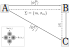
\includegraphics[width=0.8\linewidth]{qds/qds_setup}
\caption{\label{fig:qds_setup} \MT{Make a better figure. Ensure also that it is consistent with notation from the main body} Setup of the QDS protocol considered in this chapter. Alice wishes to securely sign a $1$~bit message $m$. Alice distributes quantum coherent states along insecure quantum distribution channels (solid lines) during the Distribution stage. Bob and Charlie swap eliminated signature elements via their securely encrypted classical channel (dotted lines). During the Messaging stage Alice sends a message-signature pair along a classical broadcast channel (dot-dashed line).}
\end{figure}

\MT{Chat about the setup for our signatures scheme}

Our QDS scheme is split into two stages, Distribution and Messaging, which can occur with significant time delay. The quantum states are sent and measured during Distribution, while during Messaging Alice will send her message and classical signature, and Bob and Charlie will try to determine its validity.\footnote{Note the intrinsic separation between the Distribution (quantum) and Messaging (classical) stages of the protocol. We will take further advantage of this separation between quantum and classical steps in Chapter~\MT{X}} Our protocol setup is outlined in Fig.~\ref{fig:qds_setup}, while the protocol is described in Fig.~\MT{X} \MT{I want a flowchart-style figure to outline the steps of the protocol, similar to the one which I have in 1st-year report.}



\MT{mention somewhere why we consider just a $1$ bit message}

\MT{I'll do everything for QPSK, but I should have a section where I generalize to NPSK}

\subsubsection{Distribution stage}
\noindent \underline{Step $1$.} Alice wishes to send a signed $1$ bit message $m$ to Bob and Charlie. For each possible future $m$, and for each recipient, Alice creates the following classical strings
\begin{equation}
\Phi_m^{\left(B, C\right)} = \left\{ \phi_{j, m}^{\left(B, C\right)}\right\}_{j=1}^{L}
\end{equation}
where the $\phi_{j}$ are complex phases chosen from alphabet $\mathcal{A}_4$. The $\phi_j$ are assumed to be drawn uniformly at random from $\mathcal{A}_4$, though we will relax this assumption in Chapter.~\MT{X}. The strings $\Phi_m^{\left(B, C\right)}$ are Alice's \emph{private key}. \MT{Talk somewhere about using a different private key for each recipient.} The signature length $L$ is an integer suitably chosen to ensure the desired level of security.
\par
\noindent \underline{Step $2$.} Corresponding to each of her private keys, Alice forms the following quantum states
\begin{equation}\label{eqn:QDS_publickey}
\rho\left[\Phi_m^{\left(B, C\right)}\right] := \otimes_{j=1}^L \rho\left[\phi_{j, m}^{\left(B, C\right)}\right]
\end{equation}
with
\begin{equation}
\rho\left[\phi_{j, m}^{\left(B, C\right)}\right] := \ket{\phi_{j, m}^{\left(B, C\right)}} \bra{\phi_{j, m}^{\left(B, C\right)}}
\end{equation}
understood to be the coherent state from $\mathcal{A}_4$ with phase corresponding to the relevant element of Alice's private key.

The states Eq.~\ref{eqn:QDS_publickey} may be interpreted simply as sequences of coherent states which Alice sends to each recipient. The states $\rho\left[\Phi_m^{\left(B, C\right)}\right]$ are Alice's \emph{public key}. \MT{talk somewhere about how the states she sends are different for each recipient.}
\par
\noindent \underline{Step $3$.} Each recipient $B, C$ performs heterodyne detection on each received $\rho\left[\phi_{j, m}^{\left(B, C\right)}\right]$ and receives complex phase outcome $x_{B,C}\in\mathbb{C}$. In other words, they perform the POVM
\begin{equation}
E\left[x\right] := \otimes_{j=1}^L E_j\left[x\right] \qq{with} E_j\left[x\right] := \frac{1}{\sqrt{\pi}} \ket{x}_j\bra{x}_j
\end{equation}
with $x \in \mathbb{C}$. Crucially, since measurement is performed immediately on receipt of the states, no quantum memory is required, and the remainder of the protocol is entirely classical.

At the end of the quantum stage of the protocol, recipients Bob and Charlie now each possess classical strings, length $L$, containing their complex phase measurements on Alice's distributed states, Fig.~\ref{fig:elimsig}~(a). They now form \emph{eliminated signatures}, Fig.~\ref{fig:elimsig}. For each complex outcome $x_j\in\mathbb{C}$, each recipient should record the phases $\phi_{j, m}^{\left(B, C\right)}$ which are \emph{least compatible} with $x_j$. For each element $j$, this may be understood as computing the four conditional probabilities 
\begin{equation}
p\left(\alpha_j | x_j\right) \qq{for each} \alpha_j \in \mathcal{A}_4,
\end{equation}
and recording the $\alpha_j$ giving rise to the smallest of these conditional probabilities. Note that these recorded $\alpha_j$ will always be adjacent elements of $\mathcal{A}_4$. An example of this elimination procedure is displayed pictorially in Fig.~\ref{fig:elimsig}, and for clarity we display the mapping explicitly in Tab.~\MT{X}. \MT{Create a table to illustrate the mapping to eliminated signatures.} We will denote Bob and Charlie's eliminated signatures at this stage as $X_m^{\left(B, C\right)}$. Each is of length $L$ and each will later be compared to Alice's public key in order to authenticate the message. 

\begin{figure}[htp]
\centering
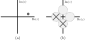
\includegraphics[width=0.8\linewidth]{qds/elimsig}
\caption{\label{fig:elimsig} \MT{(Draft)} (a) Bob and Charlie each perform heterodyne outcome on their received coherent states, and get complex outcome $x \in \mathbb{C}$. (b) They then record the two states from $\mathcal{A}_4$ which are least likely to have been sent by Alice.}
\end{figure}

\par
\noindent \underline{Step 4.} \emph{Symmetrization:} Bob and Charlie now swap a random $L/2$ elements of their $X_m^{\left(B, C\right)}$ over their secure classical channel. \MT{make sure I introduce this channel earlier}, and signature elements which have been forwarded by a player will no longer be used by him in the protocol. We denote these resulting strings as $Y_m^{\left(B, C\right)}$. Both the positions and the values of the swapped elements must be kept secret from Alice, which will ensure that the information which Bob and Charlie each hold is symmetric from Alice's point of view. 

In other words at the end of Step~$3$, having sent the state $\ket{\phi_{j, m}^B}\bra{\phi_{j, m}^B}$ to Bob, even though Alice does not know its value Alice knows that Bob holds the corresponding eliminated signature element $X_{j, m}^B$. At the end of Step~$4$ however, Alice does not know whether it is Bob or Charlie who holds $X_{j, m}^B$. This uncertainty will prove crucial for preventing her from successfully repudiating (Requirement~$3$). Bob (and Charlie) now possesses an eliminated signature $\tilde{X}_m^{\left(B\right)}$ in two halves: one half ($Y_m^{\left(B\right)}$) containing those elements received directly from Alice, and one half ($Z_m^{\left(B\right)}$)containing elements received during this Symmetrization step from Charlie.

The key parameters for the Distribution stage are the signature length $L$, which directly measures the quantum resources required for the protocol, and the alphabet parameter $\alpha$ denoting the average photon number of the distributed coherent states. Channel parameters such as loss and thermal noise will be discussed later.\footnote{We will also later discuss an extension to the protocol, and allow it to run with an $N$~PSK alphabet $\mathcal{A}_N$ of coherent states, where $N$ is an even integer.}

\subsubsection{Messaging stage}

Messaging may occur at any time after Distribution. \MT{chat about quantum memories}.

\noindent \underline{Step $5$.} To sign $m$, Alice sends to Bob the classical triplet $\Sigma = \left(m, \sigma_m\right)$, consisting of the message which she would like to convey, and her private key $\sigma_m = \left(\Phi_m^B, \Phi_m^C\right)$ which acts as $m$'s signature. 

\noindent \underline{Step $6$.} Bob rearranges $\sigma_m \rightarrow \tilde{\sigma}_m^B := \left(\tilde{\Phi}_{Y, m}^B, \tilde{\Phi}_{Z, m}^B\right)$ by selecting elements from Alice's declaration which correspond to the two halves of his eliminated signature. The original $\sigma_m$ has length $2 L$, while $\tilde{\sigma}_m^B$ has length $L$.

Bob compares elements of $\tilde{\sigma}_m^B$ to his $\tilde{X}_m^{B}$, choosing which half of $\tilde{X}_m^B$ to compare to based on whether he kept or swapped the eliminated signature element. It is as this stage that Bob makes a decision about whether to accept $m$ as genuine. His decision will be based on Alice's declared $\tilde{\sigma}_m^B$, and the number of mismatches between Alice's signature and his own eliminated signatures (see the box, ``counting mismatches").

\begin{figure}[htp]
%\centering 
\captionsetup{width=0.8\linewidth}
\begin{framed}
\noindent \underline{Counting mismatches:} a mismatch occurs if the state which Alice claims to have sent has been eliminated. To be concrete, a mismatch at position $j$ occurs when
\begin{equation}
\phi_{j, m}^B \in Y_{j, m}^B \qq{or} \phi_{j, m}^C \in Z_{j, m}^B, 
\end{equation}
and we define
\begin{equation}
\mathcal{M}\left(F, G\right)
\end{equation}
denote the probability of mismatch between an arbitrary eliminated signature $G$, and an arbitrary list of phases $F$. Both $F$ and $G$ should be of the same length.

%denote the probability of mismatch between arbitrary declared signature $F$ and arbitrary eliminated signature $G$.\MT{I think this should be more concrete}

\MT{Add an explatory figure in here}
\end{framed}
\end{figure}

If Bob measures sufficiently few mismatches on both of his eliminated signature halves, i.e. if $\mathcal{M}\left(\tilde{\Phi}_{Y, m}^B, Y_m^B\right) < s_B L/2$ and $\mathcal{M}\left(\tilde{\Phi}_{Z,m}^B, Z_m^B\right) < s_B L/2$ then he accepts Alice's declaration $m$ as genuine, otherwise the protocol aborts. The threshold $0 \le s_B \le 1$ is related to the security of the protocol and will be discussed later.

\noindent \underline{Step $7$.} If Bob has accepted $m$, then he forwards $\Sigma$ to Charlie, who similarly checks for mismatches between Alice's signature and his eliminated signature. Charlie accepts the message if $\mathcal{M}\left(\tilde{\Phi}_{Y, m}^C, Y_m^C\right) < s_C L/2$ and $\mathcal{M}\left(\tilde{\Phi}_{Z, m}^C, Z_m^C\right) < s_C L/2$, with security threshold $0 \le s_c \le 1$ to be discussed later. If Charlie also accepts $m$ then the protocol has succeeded, otherwise it aborts. 

The key parameters for the Messaging stage are $s_B, s_C$ which may be freely chosen by Bob and Charlie in order to optimize security.

%\section{Security proof}


\section{Security against repudiation}
We now turn to consider the security of the QDS protocol discussed in Sec.~\MT{X}. Recall that of the five requirements for a digital signatures protocol, requirements $3$ and $4$ are equivalent in a $3$~party setting. 

In what follows we will prove that our protocol is:
\begin{itemize}
\item secure against a repudiation attack (Requirement $3$, Fig.~\MT{X}), 
\item robust (Requirement $5$, Fig.~\MT{X}),
\item secure against a forgery attack (Requirement $1$, Fig.~\MT{X})
\end{itemize}
and we will additionally demonstrate that fulfilment of requirement $1$ implies fulfilment of requirement $2$. \MT{Make sure that I actually do this.}

Our proof will proceed by demonstrating that an attempted repudiation or forgery will induce a large mismatch rate, while a small mismatch rate is obtained when no attack is attempted. Thus, by appropriate choice of security parameters $s_B, s_C$ and signature length $L$, the probability of a \emph{successful} attack may be made arbitrarily small.

We assume that in our $3$~party setting at most \emph{one} of the players $A, B, C$ may behave dishonestly. For simplicity of notation we give a dishonest player the power to eavesdrop on the distribution of quantum states, and so the label $E$ is not required as an internal eavesdropper is at least as powerful as an external Eve. If two or more players are dishonest then we assume that they will collaborate, which allows them to trivially break the protocol. We note that a collaboration of multiple dishonest players must be considered for an $n$~party QDS protocol, as discussed in Ref.~\MT{Arrazola}, but we will not discuss it further here.

To succeed in a repudiation attack, a dishonest Alice is able to convince Bob that the message $m$ is genuine, while Charlie that $m$ is fake. Security against repudiation is guaranteed by the Symmetrization procedure (Step $4$ of the protocol) which ensures that Alice does not know which recipient holds the eliminated signature element corresponding to a particular state which she sent. The security against repudiation follows along similar lines to \MT{cite some stuff}.

We assume that Alice is free to manipulate her declared $\sigma_m = \left(\Phi_m^B, \Phi_m^C\right)$. We also assume that she may freely manipulate the number of mismatches $\mathcal{M}\left(\Phi_m^{B, C}, X_m^{\left(B, C\right)}\right)$ between her signature and the eliminated signatures $X_m^{\left(B, C\right)}$ which Bob or Charlie held before Symmetrization. We denote these mismatch rates as $p_B$ and $p_C$, respectively, and Alice may even choose them to be zero.

After Symmetrization, Bob and Charlie each possess an eliminated signature in two halves, each of length $L/2$, consisting either of elements which they received directly from Alice, or of elements which they received during this step. 

Alice succeeds in her repudiation attack if Bob accepts both of his halves as genuine, while Charlie rejects at least one of his halves as fake. That is to say, a successful repudiation attack occurs when

\begin{align}\label{eqn:repudiation_events}
&\left(\mathcal{M}\left(\tilde{\Phi}_{Y, m}^B, Y_m^B\right) < s_B L/2 \right. \notag\\
&\qq{and} \notag \\
&\left.\mathcal{M}\left(\tilde{\Phi}_{Z, m}^B, Z_m^B\right) < s_B L/2 \right) \notag \\
&\qq{and} \notag \\
&\left(\mathcal{M}\left(\tilde{\Phi}_{Y, m}^C, Y_m^C\right) \ge s_C L/2 \right. \notag \\
&\qq{or} \notag \\
&\left.\mathcal{M}\left(\tilde{\Phi}_{Z, m}^C, Z_m^C\right) \ge s_C L/2 \right) \qq{\MT{TODO: fix appearance}}
\end{align}

\noindent which we denote as events $E_A$, $E_B$, $E_C$, $E_D$, respectively. 
Thus, the probability $\varepsilon_{\text{repudiation}}$ of a successful repudiation attack is given by

\begin{equation}
\varepsilon_{\text{repudiation}} = \text{P}\left[\left(E_A \cap E_B\right) \cap \left(E_C \cup E_D\right)\right].
\end{equation}
To proceed, we require the following two probability inequalities for arbitrary events $x, y$

\begin{align}
\label{eqn:prob_inequality_1}
\text{P}\left(x \cap y\right) &\le \text{min}\left\{\text{P}\left(x\right), \text{P}\left(y\right)\right\} \\
\label{eqn:prob_inequality_2}
\text{P}\left(x \cup y\right) &\le \text{P}\left(x\right) + \text{P}\left(y\right)
\end{align}
\noindent We may now use the probability inequality Eq.~\ref{eqn:prob_inequality_1} and observe that 

\begin{equation}
\varepsilon_{\text{repudation}} \le \text{min}\left\{\text{P}\left(E_A \cap E_B\right), \text{P}\left(E_C \cup E_D\right)\right\}.
\end{equation}

\noindent Again using Eqs.~\ref{eqn:prob_inequality_1},~\ref{eqn:prob_inequality_2}, we arrive at

\begin{equation}\label{eqn:rep_prob_working}
\varepsilon_{\text{repudiation}} \le \text{min}\left\{
\text{min}\left\{\text{P}\left(E_A\right), \text{P}\left(E_B\right) \right\}, \text{P}\left(E_C\right) + \text{P}\left(E_D\right)\right\}
\end{equation}
which provides an upper bound for the probability of successful repudiation attack in terms of the individual probabilities for distinct events. We now wish to demonstrate that the probability for each event may be made arbitrarily small by suitable choice of $L$, and thus that $\varepsilon_{\text{repudiation}}$ may also be made arbitrarily small.


%\subsubsection{Bounding repudation probabilities}
We now wish to bound each of the probabilities appearing in Eq.~\ref{eqn:rep_prob_working}. We will rely on Hoeffding's inequalities Eqs.~\ref{eqn:hoeffding1},~\ref{eqn:hoeffding2} which we will use to find an upper bound for the probability that sufficiently few mismatches are observed.

We let $\mathcal{F}$ be an arbitrary string of declared phases, and $\mathcal{G}$ be an eliminated signature. We define a string $\mathcal{E}$ such that

\begin{equation*}\label{eqn:error}
\mathcal{E}_j = 
\begin{cases}
1 & \text{if $\mathcal{F}_j$ is eliminated in $\mathcal{G}_j$} \\
0 & \text{otherwise}
\end{cases}
\end{equation*}
which measures whether a mismatch has occurred between the $j^\text{th}$ elements of $\mathcal{F}$ and $\mathcal{G}$ %\footnote{Notice therefore that $(2/L)\Sigma_{j=1}^(L/2) \mathcal{E}_j = \mathcal{M}\left(\mathcal{F}, \mathcal{G}\right)$ via the mismatch function defined earlier, when $\mathcal{F}, \mathcal{G}$ each have length $L/2$.} Assume that $\mathcal{F}$ and $\mathcal{G}$ each have length $n$. Then we will bound the probability that the number of mismatches is below a threshold $s n$. 

It is easy to see that the observed mismatch rate is equivalent to the empirical mean of $\mathcal{E}$. In other words

\begin{equation}
\bar{\mathcal{E}} = \frac{1}{n} \sum_{j=1}^n \mathcal{E}_j = \mathcal{M}\left(\mathcal{F}, \mathcal{G}\right)
\end{equation}
and so we wish to bound $\text{P}\left(\bar{\mathcal{E}} \le s\right)$. Thus, we have

\begin{align}\label{eqn:qds_hoeffding1}
\text{P}\left(\bar{\mathcal{E}} \le s \right) &= \text{P}\left[\mathbb{E}\left(\bar{\mathcal{E}}\right) - \bar{\mathcal{E}} \ge \mathbb{E}\left(\bar{\mathcal{E}}\right) - s\right] \notag \\
&\le \text{exp}\left(- 2 \left[\mathbb{E}\left(\bar{\mathcal{E}}\right) - s\right]^2 n \right)
\end{align}
where the inequality follows from Hoeffding inequality Eq.~\ref{eqn:hoeffding1} provided that $\mathbb{E}\left(\bar{\mathcal{E}}\right) - s \ge 0$.

Similarly, we derive
\begin{equation}\label{eqn:qds_hoeffding2}
\text{P}\left(s \le \bar{\mathcal{E}}\right) \le \text{exp}\left( - 2 \left[s - \mathbb{E}\left(\bar{\mathcal{E}}\right)\right]^2 n\right)
\end{equation}
by applying Eq.~\ref{eqn:hoeffding2}, and again we require that \MT{condition}.

Using Eqs.~\ref{eqn:qds_hoeffding1},~\ref{eqn:qds_hoeffding2} we may now bound the probabilities for events Eq.~\ref{eqn:repudiation_events}

\begin{align}\label{eqn:qds_repudiation_events_probs}
\text{P}\left(E_A\right) \le \text{exp}\left( -\left[p_B - s_B\right]^2 L \right) \qq{provided that} p_B > s_B \notag \\
\text{P}\left(E_B\right) \le \text{exp}\left( -\left[p_C - s_B\right]^2 L \right) \qq{provided that} p_C > s_B \notag \\
\text{P}\left(E_C\right) \le \text{exp}\left( -\left[s_C - p_C\right]^2 L \right) \qq{provided that} p_C < s_C \notag \\
\text{P}\left(E_D\right) \le \text{exp}\left( -\left[s_C - p_B\right]^2 L \right) \qq{provided that} p_B < s_C
\end{align}

\noindent where in the first two inequalities we have applied Eq.~\ref{eqn:qds_hoeffding1} and in the second two inequalities we have applied Eq.~\ref{eqn:hoeffding2}. We now recall that Alice has the power to choose any $0 \le p_B, p_C \le 1$. We will consider some cases:

\noindent Assume that $p_B \ge s_B$. Then by the first inequality of Eq.~\ref{eqn:qds_repudiation_events_probs} the probability Eq.~\ref{eqn:rep_prob_working} must decay exponentially %must it? Could we decay faster? 
and so we are secure against repudiation. An analogous argument holds for the choice $p_C \ge s_B$ using the second inequality of Eq.~\ref{eqn:qds_repudiation_events_probs}.

\noindent Assume instead that $p_B < s_B$ and $p_C < s_B$. It follows that if we choose $s_B \le s_C$, then $p_B < s_C$ and $p_C < s_C$, and therefore Eq.~\ref{eqn:rep_prob_working} decays exponentially via the third and fourth inequalities of Eq.~\ref{eqn:qds_repudiation_events_probs}.

Thus, we have demonstrated the intuitive result that the choice $s_B \le s_C$ ensures that $\forall p_{B, C}$ the probability for successful repudiation is exponentially decaying. In other words, Bob's threshold for accepting the message should be stricter than Charlie's.

Let us simplify Eq.~\ref{eqn:rep_prob_working}. Clearly, increasing $p_B$ or $p_C$ will cause both of the exponentials in the first term to decrease. Because of the inner minimum, we will only care about $\text{max}\left\{p_B, p_C\right\}$, and so we define $p := \text{max}\left\{p_B, p_C\right\}$ and write

\begin{equation}
\text{min}\left\{\text{exp}\left(- \left[p_B - s_B\right]^2L\right), \text{exp}\left(- \left[p_C - s_B\right]^2L\right)\right\} = \text{exp}\left(-\left[p - s_B\right]^2L\right).
\end{equation}
We may maximise the second term of Eq.~\ref{eqn:rep_prob_working} 

\begin{equation}
\text{exp}\left(- \left[s_C - p_C\right]^2 L \right) + \text{exp}\left(- \left[s_C - p_B\right]^2 L \right) \le 2 \text{exp}\left( - \left[s_C - p\right]^2 L\right)
\end{equation}
and so

\begin{equation}
\varepsilon_{\text{repudiation}} \le \text{min}\left\{ 2 \text{exp}\left( - \left[p - s_B\right]^2 L \right), 2 \text{exp}\left( - \left[s_C - p\right]^2 L \right) \right\}.
\end{equation}
Since the minimum over two distinct Gaussians is maximized when the Gaussians have equal arguments, the probability $\varepsilon_{\text{repudiation}}$ is maximized when 
\begin{equation}
p = \frac{s_B + s_C}{2}.
\end{equation}

Finally, we reach
\begin{equation}\label{eqn:erep}
\varepsilon_{\text{repudiation}} \le 2 \text{exp}\left( - \frac{\left[s_C - s_B\right]^2}{4} L\right)
\end{equation}
as our useful bound for the probability that Alice succeeds in her repudiation attack. Since Eq.~\ref{eqn:erep} is exponentially decaying, $\forall \epsilon > 0,  \exists L$ such that $\varepsilon_{\text{repudiation}} < \epsilon$, and thus the probability can be made arbitrarily small. We are therefore secure against repudiation attack.


\section{Robustness}
The QDS protocol must be robust (Requirement~$5$, Fig.~\MT{X}) and allow the message $m$ to be accepted provided that all parties behave honestly. We would like to calculate the probability that the protocol fails in the absence of attack.

The protocol fails in the absence of attack if either Bob or Charlie rejects a message which Alice did in fact send, i.e. if Bob or Charlie detect too many mismatches on Alice's declaration $\sigma_m$. Since we have above derived that $s_B \le s_C$, it will always be more likely that Bob rejects than Charlie so we will seek to bound the probability that Bob measures more than $s_B L/2$ mismatches on either of his signature halves, and we note that this will also provide a bound for the equivalent probability at Charlie.

Let $\perr$ be the probability of honest mismatch between Alice's declaration and either of Bob's eliminated signature halves. Because of the non-orthogonality of coherent states, $p_{\text{err}} > 0$, which we will model later. Using probability inequality Eq.~\ref{eqn:prob_inequality_2}, the probability that Bob rejects either of his halves is given by

\begin{equation}
\varepsilon_{\text{Bob rejects}} \le 2 \text{P}\left(E_A\right)
\end{equation}
where $E_A$ is the event that Bob measures more than $s_B L/2$ mismatches on either of his halves. We have implicitly assumed that $\perr$ is identical between states originally sent to Bob and those originally sent to Charlie, but this is easy to relax if desired.

Using Hoeffding inequality Eq.~\ref{eqn:qds_hoeffding2} identially to the derivation of Eq.~\ref{eqn:qds_repudiation_events_probs} we see that
\begin{equation}\label{eqn:ehonabort}
\varepsilon_{\text{honest abort}} = \varepsilon_{\text{Bob rejects}} \le 2 \text{exp}\left( - \left[s_B -\perr\right]^2 L\right)
\end{equation}
provided that $\perr < s_B$. Equation~\ref{eqn:ehonabort} is our useful bound for the probability that the protocol aborts even though everyone is behaving honestly. Since it is exponentially decaying the probability that this happens can be made arbitrarily small, and so we have fulfilled Requirement~$5$.

\subsection{Modelling $p_{\text{err}}$}
\MT{let's have a figure somewhere which illustrates this}

The probability $\perr$ corresponds to the probability that a heterodyne measurement outcome $z$ has $\text{Re}\left(z\right) < 0$ when Alice distributed the coherent state $\ket{\alpha}$. In the absence of thermal noise the channel simply acts as a beamsplitter with vacuum at the fourth port, and so

\begin{equation}
|\alpha\rangle\langle\alpha| \rightarrow |\sqrt{T}\alpha\rangle\langle\sqrt{T}\alpha|
\end{equation}

\noindent when the channel has transmittivity $T$. \MT{show a derivation of this formula somewhere (either here, or in chapter~$1$.)} A heterodyne measurement on the output state gives outcome $z \in \mathbb{C}$ with probability
\begin{align}
\text{P}\left(z\right) = \langle z | \sqrt{T}\alpha\rangle\langle\sqrt{T}\alpha|z\rangle = \left|\langle z | \sqrt{T} \alpha \rangle \right|^2& \notag \\
= \frac{1}{\pi}\text{exp}\left( - \left| z - \sqrt{T}\alpha \right|^2 \right)&
\end{align}
where ket vector $|z\rangle$ denotes the coherent state centred on $z$. Then,

\begin{align}
\perr &= \text{P}\left(\text{Re}\left(z\right)<0\right) = \int\limits_{\text{Re}\left(z\right)<0}\Diff2 z \, \text{P}\left(z\right) \notag \\
&= \int\limits_{-\infty}^{\infty} \mathrm{d} y \, \text{exp}\left(-y^2\right) \int\limits_{-\infty}^{0} \mathrm{d} x \, \text{exp}\left(-\left[x - \sqrt{\frac{T}{2}}\alpha_x\right]^2\right)
\end{align}
where the factor $1/\sqrt{2}$ arises from Eq.~\MT{X} %the one relating quadratures and complex phase
and where $x = \text{Re}\left(z\right), y = \text{Im}\left(z\right)$ and $\alpha_x = \text{Re}\left(\alpha\right)$. 

Integrating, we arrive at

\begin{equation}\label{eqn:perr}
\perr = \frac{1}{2}\text{erfc}\left(\sqrt{\frac{T}{2}}\alpha\right)
\end{equation}

\noindent which models the probability of honest mismatch over a lossy channel with transmittivity $T$. The $\perr$ when the channel contains thermal noise, Fig.~\MT{X}, is given by \MT{put it here, and then talk about how it is derived and what it means.}

\section{Security against forgery}
We now turn to consider Requirement~$1$, Fig.~\MT{X}, that a QDS protocol should provide security against a forging attack. In this attack, a dishonest player (or fourth party, Eve) will declare a fake $m^\prime$ with the aim that it should be accepted by honest players as being genuine and from Alice. 

The message $m^\prime$ will have an appended signature $\tau_{m^\prime}$ consisting of declared coherent state phases, and $m^\prime$ will be accepted if $\tau_{m^\prime}$ has sufficiently few mismatches with respect to an honest player's eliminated signature. 

%Since Bob already knows $L/2$ of Charlie's elements, precisely those $Z_m^C$ which originated with Bob,

Since Bob and Charlie already know $L/2$ of each other's eliminated signature elements--those which were forwarded during the Symmetrization step of the protocol--a dishonest player who is internal to the signature scheme will have an advantage over an external Eve. Additionally, since $s_B < s_C$ it is more likely that Charlie accepts a spurious $m^\prime$ and fake signature, and so the most dangerous forger will be a dishonest Bob. We thus proceed with the mantra ``Bob is Eve'' and take Bob as our dishonest, forging party. 

Specifically, Bob's goal is to declare a string $\tilde{\Phi}^C_{Y, m^\prime}$, length $L/2$ such that 
\begin{equation}\label{eqn:forging_condition}
\mathcal{M}\left(\tilde{\Phi}^C_{Y, m^\prime}, Y_{m^\prime}^C\right) \le s_C \frac{L}{2}
\end{equation}
which will be accepted by Charlie. Bob has full control over the number of mismatches with to respect Charlie's other half signature, and can even cause there to be no mismatches if he desires.

The only way that Bob can gain information about the $Y_{m^\prime}^C$ is by eavesdropping on the distribution of states from Alice to Charlie during steps~$2$ and $3$ of the protocol, and Bob's eavesdropping attack will be fully considered in Sec.~\MT{X}, below.

Defining $\text{p}_e$ as the probability that Bob will induce a mismatch on an individual given signature element, the probability $\varepsilon_{\text{forgery}}$ that Bob succeeds in his forging attack is
\begin{equation}\label{eqn:eforg}
\varepsilon_{\text{forgery}} \le 2 \text{exp}\left( - \left[\text{p}_e - s_C\right]^2 L\right), 
\end{equation}
provided that $s_C \le \text{p}_e$. Equation~\ref{eqn:eforg} is derived using Eq.~\ref{eqn:qds_hoeffding1} similarly to Eqs.~\ref{eqn:erep},~\ref{eqn:ehonabort}. Charlie's threshold $s_C$ may be freely chosen, and by combining it with the analogous conditions required for Eqs.~\ref{eqn:erep},~\ref{eqn:ehonabort} we arrive at
\begin{equation}\label{eqn:qds_security_condition}
\perr \le s_B \le s_C \le \pe 
\end{equation}
where threshold parameters $s_B, s_C$ may be freely chosen to optimize security. 

Equation~\ref{eqn:qds_security_condition} encodes the intuitive condition that the QDS protocol is secure provided that $\pe \ge \perr$, or, in other words, that a dishonest forger will cause more mismatches than an honest player. The protocol security analysis thus relies on finding parameters and channels for which a forger is guaranteed to make too many errors, and thus for which a forging attack will be detectable. In Sec.~\MT{X} will analyse several types of eavesdropping attack which a forger can attempt, and we will derive a bound for $\pe$, allowing us to analyse protocol security.

\MT{Make a statement comparing this $\pe \ge \perr$ condition to QKD, where an eavesdropper can hide an attack below channel noise.}

\section{Signature length $L$}
\MT{Not sure yet whether I want to calculate $L$ first, or to discuss calculation of $\pe$ first. I'll write $L$ calculation just now so it is here, but I might move it later.}

We now wish to calculate the total probability $\varepsilon_{\text{fail}}$ that our QDS protocol fails by any of the routes discussed earlier: by allowing Alice to repudiate, by allowing Bob to forge, or by aborting even in the absence of attack.

For a figure of merit, we will assume that the protocol will fail in any of these ways with equal probability, and so we set
\begin{equation}
\varepsilon_{\text{fail}} = \varepsilon_{\text{honest abort}} = \varepsilon_{\text{repudiation}} = \varepsilon_{\text{forgery}},
\end{equation}
though we note that alternative combinations could be considered. Let us eliminate free parameters $s_B, s_C$ by equating the arguments of Eqs.~\ref{eqn:erep},~\ref{eqn:ehonabort},~\ref{eqn:eforg}
\begin{equation}
\left(\pe - s_C\right)^2  = \frac{1}{4}\left(s_C - s_B\right)^2 = \left(s_B - \perr\right)^2
\end{equation}
from which we may derive
\begin{equation}
s_B = \frac{3}{4} \perr + \frac{1}{4}\pe \qq{and} s_C = \frac{1}{4}\perr + \frac{3}{4}\pe
\end{equation}
as our choices of security thresholds. Notice that since $\perr \le \pe$ we automatically fulfil $s_B \le s_C$. The overall probability of failure becomes

\begin{equation}\label{eqn:efail}
\varepsilon_{\text{fail}} \le 2 \text{exp}\left( - \left[\pe - \perr\right]^2 \frac{L}{16}\right).
\end{equation}

\section{Bounding $\pe$}
To complete the security analysis of our protocol, and in order to compute an upper bound for $\varepsilon_{\text{fail}}$ Eq.~\ref{eqn:efail}, we must find an upper bound for $\pe$, the rate at which a forging Bob will induce a mismatch with respect to Charlie's signature. We will be secure provided that $\pe > \perr$. The key contribution of this section will be an upper bound for $\pe$ under two different types of forging attack

%, while fully taking into account the ambiguity in Bob's declaration.

%This ambiguity stems from the following. Because Charlie eliminates two states from $\mathcal{A}_4$, Fig.~\ref{fig:elimsig}, there are

Bob will declare a string $\tilde{\Phi}_{Y, m^\prime}^C$, length $L/2$,  which causes sufficiently few mismatches with respect to Charlie. For convenience we will abbreviate Bob's declared string as $\tilde{\Phi}^{Bob}$. Our security analysis must fully take into account the ambiguity in Bob's declarations. This ambiguity stems from the following, and is illustrated in Fig.~\MT{X}.

Because Charlie eliminates two states from $\mathcal{A}_4$, Fig.~\ref{fig:elimsig}, there are a remaining two states in $\mathcal{A}_4$ which Bob can declare without introducing a mismatch. Each of the potential two states is shared with another possible eliminated signature element, and so the probability that Bob induces a mismatch is \emph{not equivalent} to the probability that Bob misidentifies an element of Charlie's eliminated signature\footnote{And so a Helstrom-like approach \MT{define} will not work.}

This forces us to work directly in terms of mismatch probability $\pe$, which we do via our error variable $\mathcal{E}$, Eq.~\ref{eqn:error}, the $j^{\text{th}}$ element of which is $1$ if Bob induces a mismatch, and $0$ if there is no mismatch. We will continue to work in terms of QPSK alphabet $\mathcal{A}_4$, though in Sec.~\MT{X} we will show how the proof may be generalized to $\mathcal{A}_N$.

To proceed, we let $Y_j$ be the $j^{\text{th}}$ element of $Y_{m^\prime}^C$, the half of Charlie's eliminated signature based on states received directly from Alice. Bob will attempt to gain information about the $Y_j$. We write $Y_j = \left\{y_1^j, y_2^j\right\}$, with $y_1^j, y_2^j \in \mathcal{A}_4$ denoting the states which Charlie has eliminated. We note that $y_1^j$ and $y_2^j$ must be adjacent to each other in phase-space, that is, if $y_1^j = \alpha$ then $y_2^j$ must be either $i \alpha$ or $- i \alpha$. The string $\tilde{\Phi}^{Bob} = \left\{\phi_j\right\}_{j=1}^{L/2}$ is Bob's declaration, which is the result of an unspecified but optimal POVM and classical strategy.

A mismatch occurs when $\phi_j = y_1^j$ or $\phi_j = y_2^j$. Bob's average mismatch rate $\pe$ may be written in terms of $\mathcal{E}$
\begin{equation}
\pe = \text{P}\left(\mathcal{E}_j = 1\right).
\end{equation}
Because $\mathcal{E}_j$ can take one of two values, the Shannon entropy $\text{H}\left(\mathcal{E}_j\right)$ is equivalent to the binary entropy $\text{h}\left(\pe\right)$, which is defined in Eq.~\MT{X}. %define this equation in introduction chapter.

Now, consider the conditional entropy
\begin{equation}
\text{H}\left(\mathcal{E}_j, y_1^j, y_2^j \given \phi_j\right)
\end{equation}
which is related to the uncertainty about whether a mismatch has occurred under Bob's declaration $\phi_j$. Using the chain rule for conditional entropies, Eq.~\MT{X}, we write
\begin{equation}\label{eqn:qds_pe_deriv_1}
\text{H}\left( \mathcal{E}_j, y_1^j, y_2^j \given \phi_j \right) = 
\text{H}\left( \mathcal{E}_j \given y_1^j, y_2^j, \phi_j\right) + 
\text{H}\left( y_1^j, y_2^j \given \phi_j\right).
\end{equation}
Since an element $\mathcal{E}_j$ is uniquely determined once $\phi_j, y_1^j, y_2^j$ are known, we may immediately write
\begin{equation}
\text{H}\left( \mathcal{E}_j \given y_1^j, y_2^j, \phi_j\right) = 0.
\end{equation}

\noindent Using chain rule Eq.~\MT{X} once again on the left hand side of Eq.~\MT{X}, but this time expanding over variable $y_1^j, y_2^j$,
\begin{align}\label{eqn:qds_pe_deriv_2}
\text{H}\left( \mathcal{E}_j, y_1^j, y_2^j \given \phi_j \right) &=
\text{H}\left(y_1^j, y_2^j \given \mathcal{E}_j, \phi_j\right) + \text{H}\left(\mathcal{E}_j \given \phi_j\right) \notag \\
&\le \text{H}\left(y_1^j, y_2^j \given \mathcal{E}_j, \phi_j\right) + \text{H}\left(\mathcal{E}_j\right) \notag \\
&= \text{H}\left(y_1^j, y_2^j \given \mathcal{E}_j, \phi_j\right) + \text{h}\left(\pe\right)
\end{align}
where the inequality follows because conditioning cannot increase entropy, Eq.~\MT{X}.

Combining Eqs.~\ref{eqn:qds_pe_deriv_1} and \ref{eqn:qds_pe_deriv_2},

\begin{align}\label{eqn:qds_pe_deriv_3}
\text{H}\left(y_1^j, y_2^j \given \phi_j\right) &\le \text{H}\left(y_1^j, y_2^j \given \mathcal{E}_j, \phi_j\right) + \text{h}\left(\pe\right) \notag \\
&= \text{P}\left(\mathcal{E}_j=0\right) \text{H}\left(y_1^j, y_2^j \given \mathcal{E}_j=0, \phi_j\right) \notag \\
&+ \text{P}\left(\mathcal{E}_j=1\right) \text{H}\left(y_1^j, y_2^j \given \mathcal{E}_j=1, \phi_j\right) + \text{h}\left(\pe\right)
\end{align}
with
\begin{equation}
\text{P}\left(\mathcal{E}_j=0\right) = 1 - \pe \qq{and} \text{P}\left(\mathcal{E}_j=1\right) = \pe.
\end{equation}

\noindent Now, because of the ambiguity in Bob's declaration, ie. because there are two eliminated signature elements consistent with a given $\mathcal{E}_j=0$ and $\phi_j$, and since we are free to permute and relabel $y_1^j \leftrightarrow y_2^j$, we have four choices for the variable $y_1^j, y_2^j$ once $\mathcal{E}_j$ and $\phi_j$ are chosen. Thus,
\begin{equation}
\text{H}\left(y_1^j, y_2^j \given \mathcal{E}_j=0, \phi_j\right) \le \log_2 4 = 2.
\end{equation}

\noindent Additionally, since Charlie eliminates precisely half of $\mathcal{A}_4$ to form his eliminated signature, we see that
\begin{equation}
\text{H}\left(y_1^j, y_2^j \given \mathcal{E}_j=0, \phi_j\right) = \text{H}\left(y_1^j, y_2^j \given \mathcal{E}_j=1, \phi_j\right),
\end{equation}
and so Eq.~\ref{eqn:qds_pe_deriv_3} becomes
\begin{equation}\label{eqn:qds_pe_deriv_4}
\text{H}\left(y_1^j, y_2^j \given \phi_j\right) \le 2 + \text{h}\left(\pe\right).
\end{equation}

\noindent Let us expand the left hand side of Eq.~\ref{eqn:qds_pe_deriv_4} using the definition of mutual information, Eq.~\MT{X}:
\begin{equation}\label{eqn:qds_pe_deriv_5}
\text{H}\left(y_1^j, y_2^j \given \phi_j\right) = \text{H}\left(y_1^j, y_2^j\right) - \text{I}\left(y_1^j, y_2^j : \phi_j\right).
\end{equation}

\noindent There are four possible eliminated signature elements, therefore eight possible choices for $y_1^j, y_2^j$ including relabeling $y_1^j \leftrightarrow y_2^j$, and so 
\begin{equation}
\text{H}\left(y_1^j, y_2^j\right) = \log_2 8 = 3.
\end{equation}

\noindent Additionally, we lower bound Eq.~\ref{eqn:qds_pe_deriv_5} by using the fact that the Holevo information maximizes the mutual information over all POVMs 
\MT{prove this fact in ch1} 
and so
\begin{equation}\label{eqn:qds_pe_deriv_6}
\text{H}\left(y_1^j, y_2^j \given \phi_j \right) = 3 - \chi\left(y_1^j, y_2^j : \phi_j\right).
\end{equation}

\noindent Finally, combining Eqs.~\ref{eqn:qds_pe_deriv_4} and \ref{eqn:qds_pe_deriv_6} we arrive at
\begin{equation}\label{eqn:qds_hpe}
\text{h}\left(\pe\right) \ge 1 - \chi \left(y_1^j, y_2^j : \phi_j\right)
\end{equation}
which is one of our key results. The Holevo information automatically includes a dishonest Bob's optimal POVM and classical strategy.
%and so Eq.~\ref{eqn:qds_hpe} provides a good lower bound for

Since binary entropy $\text{h}\left(\pe\right)$ is monotonic for $\pe \le 1/2$, Fig.~\MT{X}, we conclude that a lower bound for $\text{h}\left(\pe\right)$ also gives us a lower bound for $\pe$. \MT{Mention/show somewhere that $\pe$ is always less than $1/2$.} The inequality~\ref{eqn:qds_hpe} may be numerically solved for Bob's mismatch rate $\pe$, which can be combined with $\perr$ in to calculate $\varepsilon_{\text{fail}}$ and provide security against collective attacks \MT{define} provided that Bob's Holevo information $\chi$ can be estimated.

\section{Attack analysis}
Let us consider several different models of Bob's eavesdropping attack. Different models will affect both the parameter regimes over which our protocol can be made secure, and the level of resources required for that security. As in the QKD literature we define the following three types of quantum attack
\begin{itemize}
\item individual: \MT{X}
\item collective: \MT{X}
\item coherent: \MT{X}
\end{itemize}
\MT{TODO: also create a figure to illustrate all of these, and provide sufficient references to the literature.}

In this Thesis we will focus on individual and collective forging attacks. Full security against coherent quantum attacks in the QKD literature has only recently been proven for the relatively simple case of the gPSK alphabet \MT{cite}, and a security proof remains tricky for the discrete modulation of coherent states. %what about Lutkenhaus papers from around 2006? What type of security do they provide?

In the QKD literature it was demonstrated \MT{cite} that under \MT{conditions}, security against the collective attack may be proven in terms of security against individual attack. \MT{demonstrate (or motivate) that the same should be true here.}

In keeping with recent trends in the QKD literature for the discrete modulation of coherent states, we will focus on bounding the attack strength of individual attack, and then use \MT{conditions} to reach security against collective attack. 

\MT{Dicuss fully the state of CV QKD security proofs, and provide a short literature review of recent developments.}

In particular, we will study both the beamsplitter attack and the entangling cloner attack for our protocol. In both of these attacks the quantum distribution channel will be replaced, by Bob and unbeknownst to Alice and Charlie, with a beamsplitter intended to mimic the effect of the channel on Charlie's measurement outcomes. In particular, Bob will either input into the channel the vacuum state, a thermal state Eq.~\MT{X}, or one arm of his two-mode entangled state Eq.~\MT{X}.

\subsection{Beamsplitter attack}
In its canonical form, the beamsplitter attack--as depicted in Fig.~\MT{X}--allows Bob to replace a lossy channel with a corresponding beamsplitter with vacuum input into the fourth port. Bob receives his quantum system from the reflected output port, and from his system he will attempt to gain information about Charlie's output. Crucially, to honest players Alice and Charlie this attack is indistinguishable from simply having a lossy transmission channel, and so all channel loss must be attributed to the action of the dishonest Bob. 

Since in the beamsplitter attack Bob inputs only vacuum into the beamsplitter's fourth port, this form of the beamsplitter attack cannot model any excess noise $\xi$ and it should therefore be ignored in the analysis. However, in order to include excess noise in our analysis, we will examine two modifications to the standard beamsplitter attack. Each modification to the standard beamsplitter attack will be discussed in turn, and then we compare all three in Fig.~\MT{X}. 

\subsubsection{\underline{$BS0$: $\xi = 0$}}
We will calculate the Holevo information $\chi$ of Bob's state after performing attack $BS0$ on the quantum channel. Attack $BS0$ is the canonical beamsplitter attack, in which Bob will replace the channel with a beamsplitter and take possession of the output of the reflected port. Crucially, the beamsplitter should be chosen such that it mimics the channel exactly, and Charlie should be unable to tell whether an attack has taken place - rather, \emph{all} loss should be attributed to Bob. Since there is vacuum input into the fourth beamsplitter port, and since no other modifications are made, this attack cannot induce any excess noise $\xi$ in Charlie's measurements, and so attack $BS0$ is useful for modelling purely lossy channels in the absence of thermal noise.

Let Alice send state $\dyad{\alpha_k}$, with the $\alpha_k \in \mathcal{A}_4$. Bob inputs the vacuum state $\dyad{0}$ into the fourth port of the beamsplitter. We will calculate the Holevo information of Bob's state $\rho_{B | C}$, which is conditioned on Charlie measuring a particular eliminated signature element.

Using beamsplitter relation Eq.~\MT{X}, we see that a beamsplitter with transmittivity $T$ enacts the following transformation on the input state
\begin{equation}
\dyad{\alpha_k}_A \otimes \dyad{0}_B \rightarrow \dyad{\sqrt{T} \alpha_k}_C \otimes \dyad{\sqrt{1-T}\alpha_k}_{B},
\end{equation}
and so Charlie holds state $\dyad{\sqrt{T}\alpha_k}$ as in the derivation of $\perr$ above, while Bob holds $\dyad{\sqrt{1-T}\alpha_k}$.

Similarly, when an arbitrary $\alpha_k \in \mathcal{A}_4$ is sent uniformly at random, we must mix over the alphabet and thus the mixed two-mode output state is
\begin{align}
\left(\frac{1}{4}\sum_{\alpha_k \in \mathcal{A}_4} \dyad{\alpha_k}_A\right) &\otimes \dyad{0}_B \rightarrow \notag \\
&\frac{1}{4}\sum_{\alpha_k \in \mathcal{A}_4} \left(\dyad{\sqrt{T}\alpha_k}_C \otimes \dyad{\sqrt{1-T}\alpha_k}_B\right).
\end{align}

\noindent Charlie heterodynes on his mode and receives outcome $c \in \mathbb{C}$, and so Bob now holds
\begin{equation}
\rho_{B | c} = \frac{1}{4}\frac{1}{\text{P}\left(c\right)}\sum_{\alpha_k \in \mathcal{A}_4} \left| \langle c | \sqrt{T}\alpha_k\rangle \right|^2 \times \dyad{\sqrt{1-T}\alpha_k}_B
\end{equation}
where $\text{P}\left(c \given \alpha_k, T\right) = \left| \langle c | \sqrt{T}\alpha_k\rangle \right|^2$ corresponds to the probability that Charlie measures $c$ on his mode given that he received state $\dyad{\sqrt{T}\alpha_k}$, while $\text{P}\left(c\right) = \sum_{\alpha_k} \text{P}\left(c | \alpha_k, T\right)$ corresponds to the total unconditional probability that he measures $c$.

Recall that the eliminated signature element held by Charlie is determined entirely by his heterodyne outcome $c$, Table.~\MT{X}. Since $\chi$ is defined in terms of eliminated signature element rather than heterodyne measurement outcome, and since many $c$ will return the same eliminated signature element, we must now mix $\rho_{B | c}$ over phase-space quadrants.

\MT{Assume I have introduced some notation for eliminated signature elements before now}

Let us consider the first eliminated signature element $e_1$. We integrate $\rho_{B | c}$

\begin{equation}\label{eqn:qds_aposterioristate}
\rho_{B | e_1} = \mathcal{N}\left(e_1\right) \int\limits_{\text{Re}\left(c\right) > 0, \; \text{Im}\left(c\right)>0} \Diff2 c \; \text{P}\left(c\right) \; \rho_{B | c},
\end{equation}
with the normalization factor defined as 
\begin{equation}
\frac{1}{\mathcal{N}\left(e_1\right)} = \int\limits_{\text{Re}\left(c\right) > 0, \; \text{Im}\left(c\right)>0} \Diff2 c \; \text{P}\left(c\right).
\end{equation}

\noindent The state $\rho_{B|e_1}$ is Bob's state when Charlie holds eliminated signature element $e_1$. Bob's states conditioned on eliminated signature elements $e_2, e_3, e_4$ are calculated likewise by varying the limits of integration.

Bob's \emph{a posteriori} entropy thus reads
\begin{equation}
S_{\text{aposteriori}} = \sum_{e_k} \text{P}\left(e_k\right) S\left(\rho_{B | e_k}\right)
\end{equation}
in terms of Von Neumann entropy $S$. In this chapter we will work in the ideal case where each eliminated signature element is equally likely, and where the entropies of each of the $\rho_{B | e_k}$ are equal, and so we simply write Bob's \emph{a posteriori} entropy as

\begin{equation}\label{eqn:aposteriori_entropy}
S_{\text{aposteriori}} = S\left(\rho_{B | e_1}\right).
\end{equation}

Bob's \emph{a priori} state is given by
\begin{equation}\label{eqn:qds_aprioristate}
\rho_{\text{apriori}} = \sum_{e_k} \text{P}\left(e_k\right) \rho_{B|e_k}
\end{equation}
with corresponding \emph{a priori} entropy simply $S\left(\rho_{\text{apriori}}\right)$. Note that the state Eq.~\ref{eqn:qds_aprioristate} is equivalent to the \emph{a posteriori} state Eq.~\ref{eqn:qds_aposterioristate} when the integration limit is extended over the entire complex plane. Finally, using
\begin{equation}
\chi = S_{\text{apriori}} - S_{\text{aposteriori}}.
\end{equation}
we calculate and plot $\chi$ under attack $BS0$ in Fig.~\MT{X}.

\subsubsection{\underline{$BS1$: $\xi > 0$}}
Next let us consider a modification to canonical attack $BS0$, displayed in Fig.~\MT{X}, which will allow for modelling of channels which induce excess noise at Charlie. In this attack, denoted $BS1$, Eve inputs a thermal state Eq.~\MT{X} into the fourth port of the beamsplitter. Let us analyse its effect on Holevo information. Its effect on Charlie's measurement outcomes is discussed above in Sec.~\MT{X} \MT{Make sure I do this}.

We wish to mix a coherent state $\rho_{\alpha_k} = \dyad{\alpha_k}$ and a thermal state $\rho_{\text{thermal}}$ on a beamsplitter with transmittivity $T$. In Fock basis our states take the following form

\begin{align}
&\rho_{\alpha_k} = e^{-\left|\alpha_k\right|^2} \sum_{n, m=0}^{\infty} \frac{\alpha_k^n \overline{\alpha_k}^{m}}{\sqrt{n! m!}} \dyad{n}{m} \notag \\
&\rho_{\text{thermal}} = \left(1 - e^{-\tilde{\beta}}\right) \sum_{p=0}^\infty e^{- p \tilde{\beta}}\dyad{p} \qq{with} \tilde{\beta} = \log_e\left(\frac{1}{\bar{n}} +1\right)
\end{align}

\noindent and so the input state into the beamsplitter is
\begin{equation}
\rho_{\text{input}} = \rho_{\alpha_k} \otimes \rho_{\text{thermal}}.
\end{equation}

\noindent Enacting beamsplitter relation Eq.~\MT{X} on $\rho_{\text{input}}$, we arrive at our two-mode output state shared between Bob and Charlie.
%\begin{align}
%%
%&\rho_{\text{output}} = \sum_{n, m, p=0}^\infty e^{- \left| \alpha_k \right|^2}\left(1 - e^{- \tilde{\beta}}\right) \frac{\alpha_k^n \overline{\alpha_k}^m}{\sqrt{n! m!}} e^{- p \tilde{\beta}} \sqrt{n! p! m! p!} \notag \\
%%
%&\sum_{k_1, k_2, l_1, l_2=0}^{n, p, m, p} \pmqty{n \\ k_1} \pmqty{p \\ k_2} \pmqty{m \\ l_1} \pmqty{p \\ l_2} \left(\sqrt{T}\right)^{k_1 + l_1} \left(\sqrt{1-T}\right)^{n + m - k_1 - l_1} \notag \\
%%
%&\left(-\sqrt{1-T}\right)^{k_2 + l_2} \left(\sqrt{T}\right)^{2 p - k_2 - l_2} \sqrt{\left(k_1 + k_2\right)! \left(n + p - k_1 - k_2\right)!} \notag \\
%%
%&\sqrt{\left(l_1 + l_2\right)! \left(m + p - l_1 - l_2\right)!}
%%
%\dyad{k_1 + k_2, n + p - k_1 - k_1}{l_1 + l_2, m + p - l_1 - l_2}
%\end{align}
%\MT{make equation prettier. And decide whether I even want to include it.}
Heterodyning on Charlie's mode using POVM Eq.~\MT{X}, we see that Bob's sub-normalized conditional state is

\MT{I think I should display Bob's sub-normalized conditional state, since I will then obviously work with it, but perhaps it is a waste of space to display the two-mode state? I can speak to NK about it}

\begin{align}\label{eqn:qds_bs1_deriv_2}
%
&\tilde{\rho}_B\left(c\right) = \frac{e^{-\left|\alpha_k\right|^2}}{\pi}\left(1 - e^{-\tilde{\beta}}\right) \sum_{n, m, p=0}^\infty \frac{\alpha_k^n \overline{\alpha_k}^m}{\sqrt{n! m!}} e^{- p \tilde{\beta}} \sqrt{n! p! m! p!} \notag \\
%
&\sum_{k_1, k_2, l_1, l_2=0}^{n, p, m, p} \pmqty{n \\ k_1} \pmqty{p \\ k-2} \pmqty{m \\ l_1} \pmqty{p \\ l_2} \left(\sqrt{T}\right)^{k_1 + l_1} \left(\sqrt{1-T}\right)^{n + m - k_1 - l_1} \notag \\
%
&\left(-\sqrt{1-T}\right)^{k_2 + l_2} \left(\sqrt{T}\right)^{2 p - k_2 - l_2} \sqrt{\left(n + p - k_1 - k_2\right)!} \notag \\
%
&\sqrt{\left(m + p - l_1 - l_2\right)!} \dyad{n + p - k_1 - k_2}{m + p - l_1 - l_2} \delta_{k_1+k_2}^{l_1+l_2} \left[ e^{-\left|c\right|^2} c^{k_1 + k_2} \overline{c}^{l_1 + l_2} \right]
%
\end{align}
\MT{make this equation pretty. Also introduce somewhere the tilde notation to convey a sub-normalized state}
where $\delta_k^l$ is the Kronecker delta which arises after tracing out Charlie's mode.

\MT{I've gotta remember to mix it over $\alpha_k$.} Now, to reach the \emph{a posteriori} state under this attack we will integrate this $\tilde{\rho}_B$, as in Eq.~\ref{eqn:qds_aposterioristate}. This will correspond to simply integrating the scalar terms involving $c$, noting that the integration operation will commute with the rest of state Eq.~\ref{eqn:qds_bs1_deriv_2}. Note also that we may neglect the $\text{P}\left(c\right)$ term from the integrand Eq.~\ref{eqn:qds_aposterioristate}, since our state is already sub-normalized by precisely the required factor. 

The integration is best performed in Polar coordinates since radial and azimuthal integrands separate. So we find
\begin{align}\label{eqn:qds_bs1_deriv_3}
\int\limits_{\text{Re}\left(c\right)>0, \text{Im}\left(c\right)>0} \Diff2 c \; &e^{-\left|c\right|^2} c^k \overline{c}^l = \notag \\
&\begin{cases}
\frac{\pi}{4} \Gamma\left(k+1\right) & \text{if } k = l \\
\frac{-i}{k-l}\left(-1 + e^{i \frac{\pi}{2}\left(k-l\right)}\right)\frac{1}{2}\Gamma\left(\frac{1}{2}\left(k + l + 2\right) \right) & \text{if } k \ne l
\end{cases}
\end{align}
with $\Gamma$ the gamma function. Indeed, the radial component of the integrand of Eq.~\ref{eqn:qds_bs1_deriv_3} is a standard integral for $\Gamma$. The final \emph{a posteriori} state is now accessible. \MT{still gotta calculate the normalization factor}

The \emph{a posteriori} state is calculated likewise, but the limits of integration should be extended to the entire complex plane. In this case,
\begin{equation}\label{eqn:qds_bs1_deriv_4}
\int\limits_{\mathbb{C}} \Diff2 c \; e^{-\left|c\right|^2}c^k \overline{c}^l = \pi \Gamma\left(k+1\right)
\end{equation}
since the polar integral forces $k=l$.


\MT{Now let us talk about how $\text{P}\left(c\right)$ is affected by noise. (first, I should understand how the heterodyne povm is derived and where factors of sqrt2 should appear)}


\MT{summary paragraph:}
The Holevo information may now be calculated in the usual way, and we compare Holevo information under different attacks in Fig.~\MT{X}.
\MT{where do I want to talk about truncating matrices and numerical methods?}

\subsubsection{\underline{$BS2$: $\xi > 0$}}
We now introduce and consider a second modification to the usual beamsplitter attack, which will allow the excess noise on the channel to be modelled. This attack can be viewed as an unphysical combination of the previous two attacks which advantages Bob and disadvantages honest parties.

As we see in Fig.~\MT{X}, below, Bob performs worse under $BS1$ than $BS0$. This is a consequence of the fact that the input noise also affects his own measurements and so will reduce his information about Charlie's output. So we modify the beamsplitter attack by imposing that the channel excess noise should only affect honest players. That is, the presence of $\xi$ causes $\perr$ to increase, but Holevo information and therefore $\pe$ should both be unaffected. 

While strictly this attack is physically inconsistent, and therefore unphysical, it is more pessimistic than either $BS0$ or $BS1$, and so the security bounds it gives are preferable to either of those attacks. The Holevo information is given by using Eqs.~\ref{eqn:qds_aposterioristate} and \ref{eqn:qds_aprioristate} in the usual way, while $\perr$ is given by Eq.~\MT{X}. The performance of this attack is analysed in Fig.~\MT{X}.

\subsection{Entangling-cloner attack}
The entangling cloner attack, depicted in Fig.~\MT{X}, is ideally suited to consistently incorporate the presence of excess noise $\xi$, and we shall see that it is a much more powerful attack than any of the beamsplitter attacks considered above. The entangling cloner attack, which we shall denote $EC$, may be viewed as a natural extension of attack $BS1$, above. Instead of inputting a thermal state into the beamsplitter's fourth port, Bob will input one arm of his entangled two-mode squeezed vacuum (TMSV) state. The mode which Bob inputs into the channel is locally indistinguishable from $\rho_{\text{thermal}}$, and so honest players cannot tell which of these attacks is being performed. 

The $EC$ attack has a long history, and is known to be the optimal collective attack for gPSK QKD \MT{cite a bunch of stuff}. Since our QPSK alphabet is non-Gaussian we make no claims as to $EC$'s optimality, though we conjecture that $EC$ will be optimal as $\alpha \rightarrow 0$, and close to optimal for $\alpha << 1$. The status of optimal attacks on QDS is an open one and should be the subject of further exploration. The question about optimal attacks on QKD with discrete modulated coherent states is also open, despite a long history of activity on these protocols. In any case, the $EC$ attack is very difficult to perform with today's technology, and so a protocol with security against $EC$ (or even $BSx$) attacks should be expected to be practically secure for a long time.

\MT{Talk somewhere about where the extra power in the EC attack comes from - we allow Bob to exploit also the correlations between his two modes. Also have some figures of histograms of this attack}

Let us analyse the $EC$ attack. Alice creates the coherent state $\rho_{\alpha_k}$ (Eq.~\MT{X}), while Bob creates
\begin{equation}
\tmsv = \frac{1}{\cosh^2 \zeta}  \sum_{n, m=0}^\infty \left(\tanh\zeta\right)^{n+m} \dyad{n, n}{m, m}.
\end{equation}

\noindent Let us write the three-mode input state to the channel as

\begin{align}
\rho_{\text{input}} &= \frac{e^{-\left|\alpha_k\right|^2}}{\cosh^2 \zeta} \sum_{n_1, m_1=0}^\infty \sum_{n_2, m_2=0}^{\infty} \frac{\alpha_k^{n_1} \overline{\alpha_k}^{m_1}}{\sqrt{n_1! m_1!}} \left(\tanh\zeta\right)^{n_2 + m_2} \notag \\
&\times \bigg[\dyad{n_1, n_2}{m_1, m_2}\bigg] \otimes \dyad{n_2}{m_2}
\end{align}

\noindent where we have explicitly separated in square brackets the two modes which will interfere on the beamsplitter.

The beamsplitter mixes $\dyad{n_1, n_2}{m_1, m_2}$ via Eq.~\MT{X}, and gives an entangled three-mode state at the output. Charlie heterodynes on his mode and receives outcome $c$, and we arrive at Bob's sub-normalized two-mode output state:

\begin{align}\label{eqn:qds_ec_deriv_1}
&\tilde{\rho}_{B}\left(c\right) =  \frac{e^{-\left|\alpha_k\right|^2}}{\cosh^2\zeta} \frac{1}{\pi} \sum_{n_1, m_1, n_2, m_2 = 0}^\infty \alpha_k^{n_1} \overline{\alpha_k}^{m_1} \left(\tanh\zeta\right)^{n_2 + m_2} \sum_{k_1, k_2, l_1, l_2 = 0}^{n_1, n_2, m_1, m_2}  \notag \\
%
&\sqrt{n_2! m_2!} \left(\sqrt{T}\right)^{k_1 + l_1} \left(\sqrt{1-T}\right)^{n_1 + m_1 - k_1 - l_1} \left(-\sqrt{1-T}\right)^{k_2 + l_2} \left(\sqrt{T}\right)^{n_2 + m_2 - k_2 - l_2} \notag \\
%
&\times \sqrt{\left(n_1 + n_2 - k_1 - k_2\right)! \left(m_1 + m_2 - l_1 - l_2\right)} \notag \\
%
&\times \left[k_1! k_2! l_1! l_2! \left(n_1 - k_1\right)! \left(n_2 - k_2\right)! \left(m_1 - l_1\right)! \left(m_2 - l_2\right)! \right]^{-1} \notag \\
%
&\times \dyad{n_1 + n_2 - k_1 - k_2}{m-1 + m_2 - l_1 - l_2} \otimes \dyad{n_2}{m_2} \notag \\
%
&\times \left[e^{-\left|c\right|^2} c^{k_1 + k_2} \overline{c}^{l_1 + l_2} \right]
\end{align}

\noindent where we have again separated the terms involving $c$. Once again the state is readily integrated in $c$, either over the entire complex plane or a single quadrant, and we may simply substitute Eqs.~\ref{eqn:qds_bs1_deriv_3},~\ref{eqn:qds_bs1_deriv_4} into Eq.~\ref{eqn:qds_ec_deriv_1} to reach the \emph{a posteriori} and \emph{a priori} states, respectively.

The \emph{a priori} state is automatically normalized by virtue of the integration over $\mathbb{C}$, while the \emph{a posteriori} state is normalized by multiplying by

\begin{equation}
\frac{1}{\mathcal{N}\left(e_1 \given \xi\right)} = \int\limits_{\text{Re}\left(c\right) > 0, \; \text{Im}\left(c\right)>0} \Diff2 c \; \text{P}\left(c \given \xi \right).
\end{equation}
where we have included excess noise $\xi$ in our probability, as in Eq.~\MT{X}.















